\chapter{BitHoc: Implementation on real mobile handhelds}
\label{chapter:Bithoc}
\minitoc
Content sharing is currently a universal concern among computer users and has recently become an important requirement for mobile handhelds. Indeed, thanks to the efficient wireless connectivity offered by mobile devices (PDAs, smartphones...), users are frequently brought to locate and share content of interest (data, photos, videos, etc) with other members of the same spontaneous community. 

With current technology, they are mainly using point-to-point basic connections, which can be considered as an efficient solution when the number of users interested in the sharing session is very small. However, in the case of a large community (for example, mobile handheld users assisting to a conference and willing to share some papers), one is facing the following problem: Increasing the number parallel point-to-point communications may decrease the global ad hoc network capacity, while increasing dramatically the download time. The multi-hop point-to-point communication over long paths is also a serious issue. Therefore, there is a strong need to organize the communication overlay among nodes in a way to distribute fairly the burden of data sharing among the set of participants while aiming to decrease the global download time. P2P file sharing solutions are good candidates for such infrastructureless networks as they are based on multi-sourcing which balances resource consumption among peers and reduces the dependency on any central entity. But unfortunately, P2P content sharing applications developed for the Internet cannot directly be plugged and used into mobile devices. Indeed, on one hand, these solutions are not adapted to the constraints of multi-hop wireless networks. For example, it is known that in a resource constrained environment, the choice of the peers to whom to connect cannot be done independently of information on the underlying dynamic topology. Moreover, centralized peer management approaches like the tracker used in BitTorrent do not perform well in such environment as the tracker can be either far away or even invisible by some peers because of disconnections. Furthermore, computer users rely on Internet search engines and dedicated desktop applications to look for the content they are willing to share. This approach becomes obsolete in the case of a spontaneous MANET based community and thus, a dedicated distributed content discovery approach must be provided. One has to add the fact that from a technical point of view, limited Software Development Kits (SDK) proposed for mobile handhelds represent only a sub-set of classical SDK(s) used for desktops which leads to incompatibility problems.

This chapter presents BitHoc, an open-source standalone software solution for content sharing in MANETs that overcomes the aforementioned challenges. This software is downloable from our web site \cite{Bithoc} and has been presented in different demonstration sessions of international conferences \cite{MOBIHELD}\cite{PERCOM}. The architecture of BitHoc consists of three main components: a content discovery service (BitHoc Search Engine), a membership management service (distributed BitHoc Tracker) and a content sharing service (BitHoc Client). BitHoc tracker agents installed in nodes connect to each other in order to form and manage the per-content sharing overlay needed by the BitHoc client. This emulates the central tracker of standard BitTorrent. They also construct the content discovery overlay used by the BitHoc search engine to enable content publishing and discovery. To connect to a sharing overlay, a node needs to retrieve a torrent file (a meta-data file) by connecting to the discovery overlay. The members of this overlay manage a distributed database that contains for each torrent the list of nodes uploading it and a short description of the related content. To ensure content sharing, the BitHoc client decides, using routing information available at layer 3, of the structure of the data exchange overlay seen by him (with whom to exchange data). It also manages the scheduling of data pieces among devices. Our main contribution here is to adapt the peer neighbor and piece selection strategies of BitTorrent to account for the topology of the network and for the scarcity and shared nature of resources. The algorithms used in these three components of BitHoc are inspired from those presented in chapters \ref{chapter:membership} and \ref{chapter:content}.

We developed our software on mobile devices having Windows Mobile 6 \cite{WM6} as an operating system and equipped with WIFI adapters. As permanent topology information is required by BitHoc, we chose to use the proactive routing protocol OLSR \cite{MOLSR}. For the evaluation, we measured the performance of BitHoc with regard to the download time and sharing ratio metrics. Our test-bed allows us to experiment with the different features of our solution and to compare our version of the BitTorrent's algorithms to the ordinary Internet one when deployed in a wireless ad hoc environment. The performance analysis based on experimentation shows that BitHoc outperforms the standard version, which is in compliance with what has been shown throughout this thesis. 

The remainder of this chapter is organized as follows. Section \ref{secreq} analyses the objectives of BitHoc. Section \ref{secarchitecture} describes its architecture. Section \ref{sectest} presents the test-bed we have used to test and evaluate our solution and we show some results.


\section{Requirements Analysis}
\label{secreq}
 We designed our package in such a way to be standalone. So, the user has just to install the software to start publishing and discovering contents and sharing them later with those having the same interest. The wireless nodes not interested by the same content collaborate by forwarding packets at the routing level. Through BitHoc, we provide solutions to the following problems:
\begin{itemize}
\item{In the classical version of BitTorrent \cite{BitTorrentW}, peers periodically contact a central rendezvous point called Tracker to obtain fresh information about the peers interested in a specific content and to update their information on the progress of the download. This membership information is dynamic since peers can join and leave the content sharing overlay (called torrent) at any time during the session. Because of the inappropriateness and the large overhead of client/server architectures in wireless ad hoc networks, it is important to introduce a distributed Trackerless solution to manage the membership of the sharing session. The BitHoc tracker component of our architecture is designed for this purpose and is inspired from the membership management protocol we presented in details in Chapter \ref{chapter:membership}.}
\item{The classical version of BitTorrent \cite{BitTorrentW} supposes that the cost of sending data packets to peers is in somehow independent of their locations. In an ad hoc network, performance metrics like achievable throughput, delay, and energy consumption strongly depend on the number of hops to the peer node. So, it is clearly suboptimal and even unrealistic to deal with peers without considering the underlying topology. Furthermore, when applying the classical BitTorrent incentives in a wireless multi-hop network, nodes fail to reciprocate data fairly among them. The content dissemination scheme is close to a wave transferring data from the initial seed to the farthest peers. Through new peer selection and content piece scheduling strategies, our solution is topology-aware and ensures fair sharing. These strategies are described in details in Chapter \ref{chapter:content}.}
\item{To join a sharing session, a user should find and download the Torrent file related to that session. In the Internet, peers usually find their torrent files by the help of search engines which mainly look for the files in different central servers. This method does not apply in a mobile ad hoc environment as MANETs. The BitHoc search engine overcomes this challenge by maintaining a distributed torrent file database thanks to the overlay constructed by the BitHoc Tracker.}
\end{itemize}
\section{Architecture of BitHoc}
\label{secarchitecture}
In this section, we describe the architecture of the BitHoc application. Figure \ref{figarch} depicts the principal components of this architecture and the interactions between them. We illustrate these interactions through three typical usage scenarios:
\begin{figure}[!htbp]
  \begin{center}
    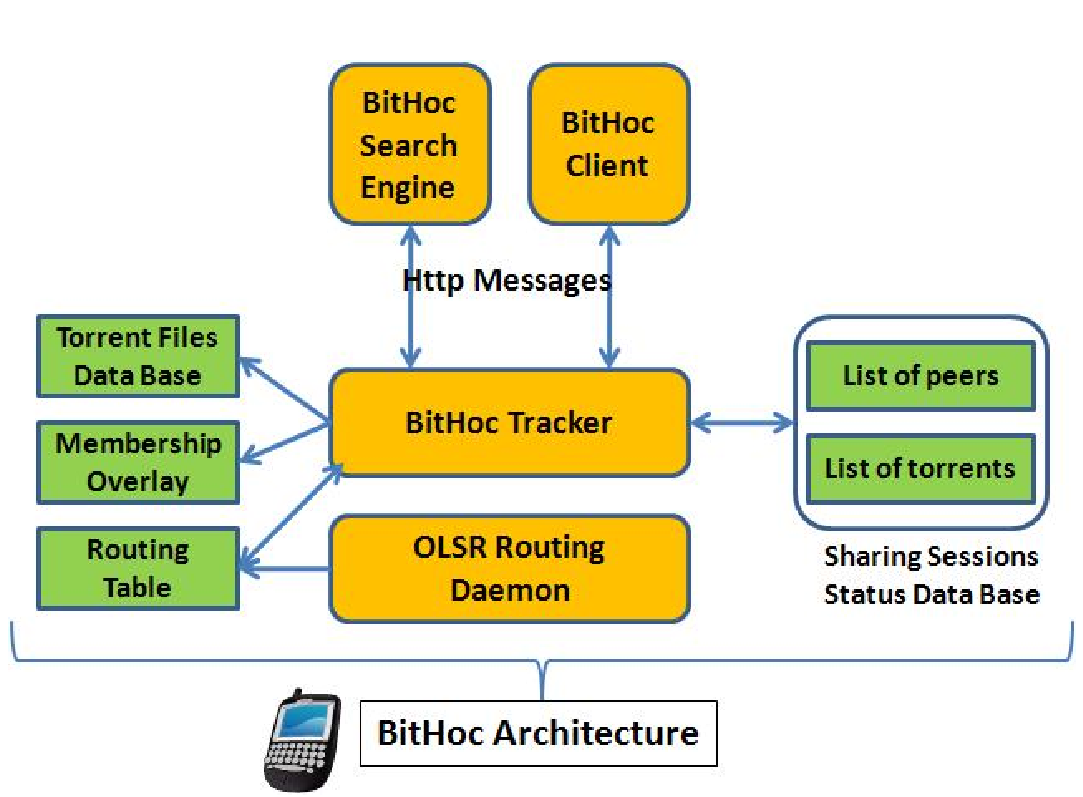
\includegraphics[width=0.7\textwidth]{Chapitre6/architecture.png}
  \end{center}
  \caption{Architecture of BitHoc}
  \label{figarch}
\end{figure}

\subsection{Content publishing and discovery}
A user willing to share some content with the members of his community needs to indicate to the BitHoc client the location of the content in the mobile device file system. First, the client creates a meta-info file (Torrent file) that identifies in a unique manner a sharing session for this specific content. After that, the user publishes (locally) the new torrent file and a short text description of the related content using the BitHoc Search Engine service, which will update the local Torrent file database maintained in the underlying BitHoc Tacker via HTTP messages. A remote user, willing to share the same content, has to use the BitHoc search engine to find and download the Torrent file. He specifies for that the name of the content or some keywords related to its description. The request is sent via HTTP messages to its local tracker which looks for the closest match in its local database. If there are no matches, it forwards the HTTP request to the other trackers in the discovery overlay. Then, it presents the received results through an ergonomic user interface (see Figure \ref{Figsearchengine}). Based on the details of received answers (fitness to the search, number of peers involved in the sharing session, number of seeders, and number of lechers, etc), the user can choose the torrent file to download, then start sharing the content using the BitHoc Client.

\begin{figure}[!htbp]
  \begin{center}
    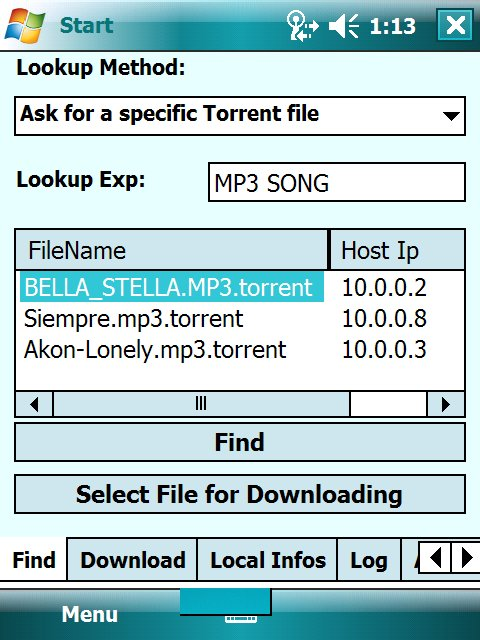
\includegraphics[width=2in,height=3in]{Chapitre6/searchengine.png}
  \end{center}
  \caption{Search Engine screen shot}
  \label{Figsearchengine}
\end{figure}

\subsection{Membership management}
When a peer wants to join or leave the sharing session, the BitHoc client informs the BitHoc Tracker about this event using a specific HTTP message. This local agent disseminates this modification to the other BitHoc Tracker agents in other nodes in order to update their knowledge about the global membership information. The communications between Tracker agents are established in an event-driven fashion and use HTTP messages. Each tracker holds a HTTP server accepting HTTP requests from other agents and from the local BitTorrent client. The BitHoc Tracker component receives from the routing daemon up-to-date routing entries. In our testbed, the dynamics of the ad hoc network are captured by the OLSR routing protocol \cite{MOLSR}. Each time the number of hops toward a given peer changes, the routing daemon fires an event, which will be caught by the BitHoc Tracker and forwarded internally to the BitHoc client. This way we are sure the peer selection strategy always uses the updated number of hops to other peers. The parameters of the communications among tracker agents like HTTP listening ports and IP addresses can easily be configured by users via an ergonomic GUI. In addition to these functionalities, the BitHoc Tracker allows the user to monitor in real-time the status of the overlay (Contents it shares, members of the session, current topology of the ad hoc network). He can even decide to keep traces about all the events in a file. For this, he just needs to activate the tracing option provided by the application.

\subsection{Content sharing}
Before starting a new sharing session, the user can choose between two versions of BitTorrent algorithms: The classical version \cite{BitTorrentW} and our version adapted to mobile ad hoc networks described in Chapter \ref{chapter:content}. The BitHoc client offers a Wizard allowing the user to configure the parameters of BitTorrent (communication ports, choking slot duration, minimum and maximum number of peers, etc). Once the torrent file is obtained, the BitHoc client can start the sharing session where it can either play the role of a leecher or a seed. It contacts periodically the local BitHoc tracker to get the current list of members of the same content sharing session (torrent). Using this list and the routing table, it manages the connections with the interested peers. Briefly a client implementing our algorithms exchanges pieces with close peers and only seeds distribute pieces across the network. Note that we allow the user to pause or resume the download while conserving the session context. He can also monitor in real time the status of the session (downloaded bytes, uploaded bytes, numbers of leechers, number of seeders, elapsed time, etc). Furthermore, the BitHoc client keeps in a log file statistics on the content sharing session and provides different levels of event traces. It also manages the storage of the downloaded contents and their classification. Figure \ref{Figclient} shows a screenshot of the BitHoc client.

\begin{figure}[!htbp]
  \begin{center}
    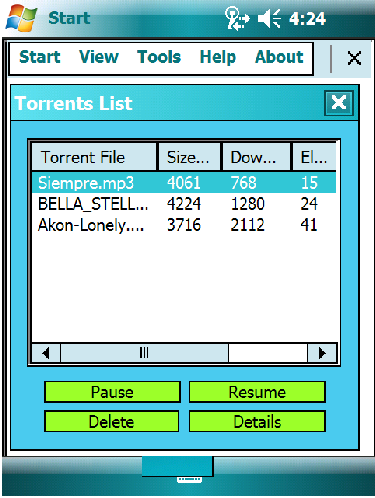
\includegraphics[width=2in,height=3in]{Chapitre6/contentsharing.png}
  \end{center}
  \caption{BitHoc Client screen shot}
  \label{Figclient}
\end{figure}


\section{Experimentation and results}
\label{sectest}
\subsection{Test-bed description}
Our wireless ad hoc network experimental environment consists of 14 mobile devices including 7 PDAs (HP iPAQ 214) and 7 smartphones (HP iPAQ 614c). Each handheld is equipped with an IEEE802.11b wireless card. The characteristics of the two types of devices are detailed in Table \ref{tabcarac}. The ad hoc connectivity is maintained thanks to OLSR daemons run by the different devices. In our experiments, we constructed several network topologies containing a maximum of 6 hops. The objective of the realized swarm was to download a 4 MB MP-3 content. All PDAs were supposed to participate to the sharing of the file. The original seed of the content was chosen randomly among the set of the 14 PDAs.
\begin{table}[h!]
\center
\label{tabcarac}
\caption{Characteristics of mobile handhelds}
\begin{tabular}{|l|c|c|}
  \hline
   & \textbf{PDA} & \textbf{Smartphone} \\
  \hline
  \textbf{Name} & HP iPAQ 214 & HP iPAQ 614c\\
\hline
  \textbf{Processor speed} & 624 MHz & 520 MHz \\
  \hline
\textbf{RAM} & 128 MB & 128 MB \\
  \hline
\textbf{Operating system} & Windows Mobile 6 & Windows Mobile 6 \\
  \hline
\end{tabular}
\end{table}

\subsection{Experimentation results}
\begin{figure}[!htbp]
  \begin{center}
    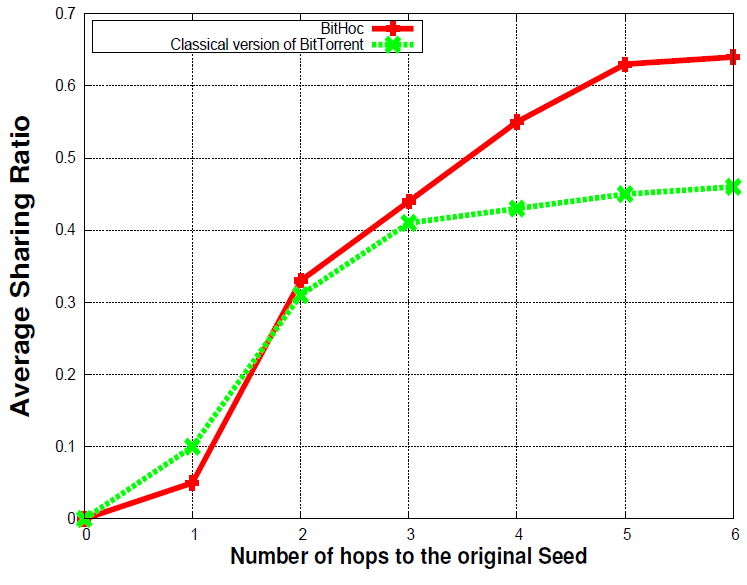
\includegraphics[width=3in,height=2.2in]{Chapitre6/sharingratio.png}
  \end{center}
  \caption{Sharing ratio}
  \label{figsharing}
\end{figure}

\begin{figure}[!htbp]
  \begin{center}
    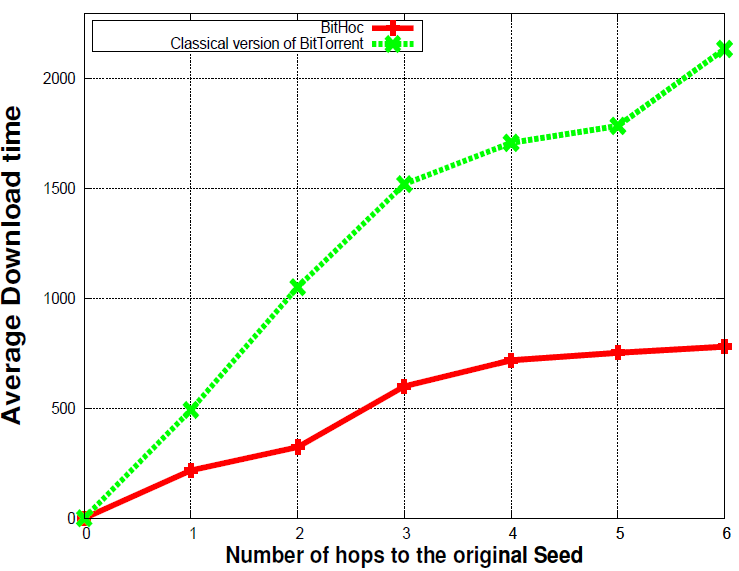
\includegraphics[width=3in,height=2.2in]{Chapitre6/downloadtime.png}
  \end{center}
  \caption{Download time}
  \label{FigDownloadtime}
\end{figure}
The metrics tracked during our experiments are the download time and the average sharing ratio of nodes. We define $R_{h}$ as the sharing ratio of peers located at $h$ hops from the original seed. It measures the level of reciprocity between downloads and uploads. In the ideal case, the ratio should be close to 1. The two versions of BitTorrent (The legacy one and ours) have been tested and the results are presented in Figures \ref{figsharing} and \ref{FigDownloadtime}. Figure \ref{figsharing} shows a dramatic increase of sharing opportunities when our adapted version is deployed. The routing overhead generated by the classical version makes any gain obtained by important diversification of pieces negligible. Our method finds the good equilibrium between sharing and diversification. Figure \ref{FigDownloadtime} shows that BitHoc outperforms the classical version of BitTorrent in terms of download time. It is in accordance with our research results presented in chapter \ref{chapter:content}. More information about our experiments and our GPL licensed open-source code can be found on the BitHoc web site \cite{Bithoc}.

\section{Conclusions and perspectives}
In this Chapter, we described our solution for content sharing in wireless ad hoc networks. The implementation that we have proposed contains three components: a distributed membership management service, a content search engine and an optimized content sharing service. The design of these services takes into consideration the constraints of mobile environments and the user needs. With the help of a real test-bed composed of PDAs and Smartphones, we were able to validate our solution in a real scenario and to compare it to other classical approaches. The experiments show that our application outperforms the classical approach and highlight the utility of its features. In particular, we were able to reduce by a factor of 2 to 3 the download time and to increase dramatically the sharing ratio. As a perspective, we plan to implement the application on other types of devices and do extensive experiments with real users.

